% Copyright 2004 by Till Tantau <tantau@users.sourceforge.net>.
%
% In principle, this file can be redistributed and/or modified under
% the terms of the GNU Public License, version 2.
%
% However, this file is supposed to be a template to be modified
% for your own needs. For this reason, if you use this file as a
% template and not specifically distribute it as part of a another
% package/program, I grant the extra permission to freely copy and
% modify this file as you see fit and even to delete this copyright
% notice.

\documentclass[t]{beamer}

% There are many different themes available for Beamer. A comprehensive
% list with examples is given here:
% http://deic.uab.es/~iblanes/beamer_gallery/index_by_theme.html
% You can uncomment the themes below if you would like to use a different
% one:
%\usetheme{AnnArbor}
%\usetheme{Antibes}
%\usetheme{Bergen}
%\usetheme{Berkeley}
%\usetheme{Berlin}
%\usetheme{Boadilla}
%\usetheme{boxes}
%\usetheme{CambridgeUS}
%\usetheme{Copenhagen}
%\usetheme{Darmstadt}
%\usetheme{default}
\usetheme{Frankfurt}
%\usetheme{Goettingen}
%\usetheme{Hannover}
%\usetheme{Ilmenau}
%\usetheme{JuanLesPins}
%\usetheme{Luebeck}
%\usetheme{Madrid}
%\usetheme{Malmoe}
%\usetheme{Marburg}
%\usetheme{Montpellier}
%\usetheme{PaloAlto}
%\usetheme{Pittsburgh}
%\usetheme{Rochester}
%\usetheme{Singapore}
%\usetheme{Szeged}
%\usetheme{Warsaw}


%remove the icon
%\usefonttheme[onlylarge]{structuresmallcapsserif}

\title{Using Past Speaker Behavior to Better Predict Turn Transitions}

\author{Tomer Meshorer \and Peter A Heeman}
% - Give the names in the same order as the appear in the paper.
% - Use the \inst{?} command only if the authors have different
%   affiliation.

\institute[] % (optional, but mostly needed)
{
  \inst{}
 Center for Spoken Language Understanding\\
 Oregon Health \& Science University, Portland, Oregon,USA
 }
% - Use the \inst command only if there are several affiliations.
% - Keep it simple, no one is interested in your street address.

\date{Interspeech, 2016}
% - Either use conference name or its abbreviation.
% - Not really informative to the audience, more for people (including
%   yourself) who are reading the slides online

%\subject{Theoretical Computer Science}
% This is only inserted into the PDF information catalog. Can be left
% out.

% If you have a file called "university-logo-filename.xxx", where xxx
% is a graphic format that can be processed by latex or pdflatex,
% resp., then you can add a logo as follows:

% \pgfdeclareimage[height=0.5cm]{university-logo}{university-logo-filename}
% \logo{\pgfuseimage{university-logo}}

% Delete this, if you do not want the table of contents to pop up at
% the beginning of each subsection:
\AtBeginSubsection[]
{
  \begin{frame}<beamer>{Outline}
    \tableofcontents[currentsection,currentsubsection]
  \end{frame}
}

% Let's get started
\begin{document}

\begin{frame}
  \titlepage
\end{frame}

\begin{frame}{Outline}
  \tableofcontents
  % You might wish to add the option [pausesections]
\end{frame}

% Section and subsections will appear in the presentation overview
% and table of contents.
\section{Motivation}
%slide 1%
\begin{frame}{Problem and Thesis}
  \begin{itemize}
  \item For a natural conversation between human and machine, we want to conform
        to human to human turn taking system (Sacks et al, 1978)
  \item In Human-Human conversations conversant predict (Sacks et al, 1978) or 
        signal (Duncan 1972) each other on coming turn transition
  \item {
    Timeouts leads to poor user interaction(Arsikere et al, 2015)
    \begin{itemize}
        \item Not effective in noisy environment
        \item too little - machine barge in during intra turn pause.
        \item too much - user waiting for the machine.
    \end{itemize}
  }
  \item {
    Turn transition prediction based on local features improve turn taking but still
    do not match human performance.
    \begin{itemize}
        \item Syntactic (Sacks et al 1978,De Ruiter et al. 2006)
        \item Prosodic (Ford 1996,Stolcke 2002,Ferrer 2003) 
        \item Pragmatic (Ford 2001)
    \end{itemize}
  }
  \end{itemize}
\end{frame}

\begin{frame}
  \begin{block}{Goal of Work}
   Use summary features which are computed over the speaker history in
   the conversation to better predict turn transition.
  \end{block}
\end{frame}



%slide 2
\begin{frame}{Conversation}

\begin{figure}
 \centering
 \includegraphics[scale=0.3]{c2.png}
 \end{figure}

  \begin{block}{Conversation}
    { $\ldots  s_{i-2}, d_{i-2}, s_{i-1} , d_{i-1}, s_i, d_i  \ldots$  }
  \end{block}
  \begin{block}{Conversation with turn change}
     $\ldots d_{i-2}, y_{i-1}, d_{i-1}, y_{i} , d_i, y_{i+1}\ldots$
  \end{block}
\end{frame}

\section{Summary Features}

%slide 3
\begin{frame}{Relative Turn Length}
\begin{itemize}
  \item Measure how long (in percent) the current turn length relative to his/her average turn length.
  \item {Computed as follow:
        \begin{itemize}
            \item $S_i$ to be the set of complete turns of speaker $s_i$ that are prior to the turn that $d_i$ is in.
            \item compute the average turn length up to the last turn
                \begin{block}{Average turn length }
                   $avg\_t_i = \frac{\sum_{t \in S_i} length(t)}{|S_i|}$
                \end{block}
            \item Compute relative turn length at the end of each dialog act
                \begin{block}{Relative Turn Length}
                     $rt_i =  \frac{length(t_i)} {avg\_t_i}$
                \end{block}
         \end{itemize}
         }
\end{itemize}
\end{frame}

\begin{frame}{Relative Turn Length}
 \begin{figure}[ht!]
 \centering
 \includegraphics[width=0.5\textwidth,width=8cm,height=8cm,keepaspectratio]{rl1.png}
 \caption{Relative turn length\label{overflow}}
 \end{figure}

\end{frame}

\begin{frame} {Relative Floor Control}
\begin{itemize}
    \item Measure how long (in percent) the current speaker held the conversation floor. How dominate he/she is.
    \item Computed as follow:
         \begin{itemize}
              \item compute the total conversation time.
                 \begin{block} {Total Conversation Time}
                       $c_i = \sum_{t \in S_i \cup L_i} length(t)$
                 \end{block}
             \item  compute the total time of the current speaker relative to the total conversation time
                 \begin{block}{Relative Floor Control}
                     $\frac{\sum_{t \in S_i} length(t)} {c_i}$
                 \end{block}
         \end{itemize}
 \end{itemize}        
\end{frame}        

\begin{frame} {Relative Floor Control}
\begin{figure}[ht!]
\centering
 \includegraphics[width=0.5\textwidth,width=8cm,height=8cm,keepaspectratio]{relative_control.png}
 \caption{Relative floor control\label{overflow}}
 \end{figure}
\end{frame}



\section{Evaluation}

% slide 5

\begin{frame}{Preprocessing}
  \begin{itemize}
    \item Removed 11 dialogue acts that were coded as other in switchboard.
    \item Skip the first 120 seconds of the conversation. 
      \begin{itemize}
      \item Gives time for conversant to form the conversional image. 
      \item Reduces the dialogue acts from 50633 to 37508.
      \end{itemize}
    \item Reduce data sparsity by collapsing 65 dialog acts into 9.
  \end{itemize}

  \begin{table}
     \begin{center}
     \begin{tabular}{l | l}
    \hline
Switchboard dialog acts &  Dialog act classes  \\
    \hline
sd,h,bf      & statement   \\
sv,ad,sv@    & statement - opinion  \\
aa,aa\^r     & agree accept \\
\%.\%-,\%@   & abandon      \\
b,bh         & backchannel  \\
qy,qo,qh     & question     \\
no,ny,ng,arp & answer       \\
+            & +            \\
o@,+@        & NA           \\
  \hline
\end{tabular}
\end{center}\vspace{-0.5em}
\caption{Mapping from dialog act to dialog act class}
\label{tab:mapping}
\end{table}
\end{frame}


\begin{frame}{ML Classifiers}
  \begin{itemize}
  \item Used random forests (N=200) to train and test the following models
  \begin{itemize}
    \item baseline 1: current dialog act label.
    \item baseline 2: current and previous dialog acts.
    \item summary model: just the summary features.
    \item full model: summary features and the current and previous dialog acts.
  \end{itemize}
  \item Evaluation was done using 10 fold cross validation. 
  \item Run grid search to find the optimal hyper parameters. 
  \end{itemize}
\end{frame}

% slide 4
\section{Results and Discussion}

\begin{frame}{Accuracy}
\begin{table}
\begin{center}
 \begin{tabular}{| l | l | l | c |}
    \hline
    Model & Accuracy & AUC & hyper parameters\\
    \hline
    Baseline 1      & 60.26\% & 0.63 & \scriptsize{max\_features=sqrt, max\_depth=7} \\
    Baseline 2     & 74.43\% & 0.79 & \scriptsize{max\_features=log2, max\_depth=9}\\
    Summary        & 66.14\% & 0.65 & \scriptsize{max\_features=sqrt, max\_depth=5} \\
    Full           & 76.05\% & 0.82 &\scriptsize{ max\_features=10, max\_depth=9}\\
  \hline
\end{tabular}
\end{center}
\caption{Accuracy, Area under the curve }
\end{table}
\begin{itemize}
\item Using only summary features is more accurate than Baseline 1.
\item The Full model is more accurate than Baseline 2.
\end{itemize}

\end{frame}



\begin{frame}{ROC curves and AUC of the different models}
 \begin{figure}[ht!]
 \centering
 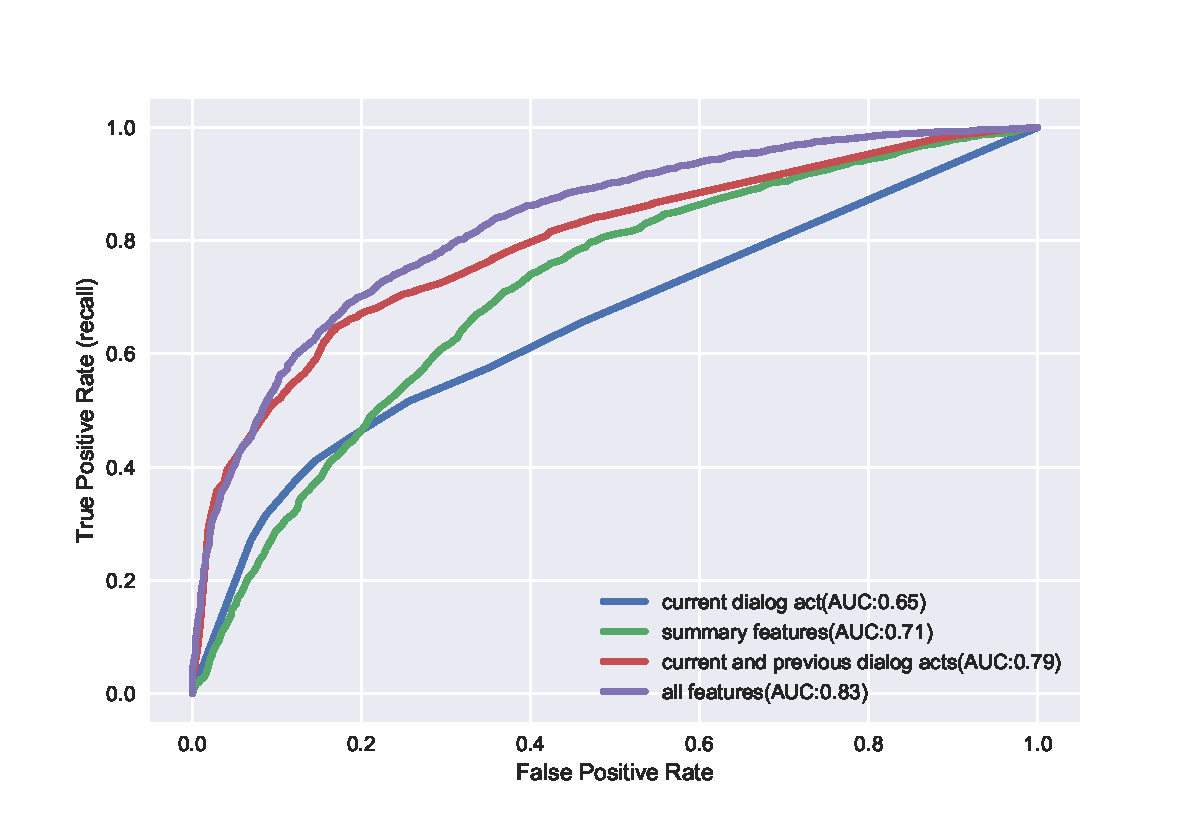
\includegraphics[width=8cm,keepaspectratio]{roc.pdf}
 \end{figure}

\end{frame}


\begin{frame}{Precision \& Recall}

\begin{table}
   \begin{center}
    \begin{tabular}{|l|l|l|c|}
    \hline
    Model & Precision & Recall & F1\\
    \hline
    Baseline 1               &69.49\% &45.52\%&54.97\%\\
    Baseline 2               &80.38\% &68.80\%&74.08\%\\
    Summary                  &64.55\% &68.88\%&66.42\%\\
    Full                     &76.17\% &77.25\%&74.87\%\\
  \hline
\end{tabular}
\end{center}
\caption{Precision, recall and F1 results }
\end{table}
\begin{itemize}
    \item Summary model makes more mistakes vs Baseline 1, however it detects more turn transition.
    \item Summary model makes more mistakes vs Baseline 2
    \item Full model makes slightly more mistakes vs Baseline 2, however it detects more turn transitions. Overall F1 is slightly better.
\end{itemize}
\end{frame}




% Placing a * after \section means it will not show in the
% outline or table of contents.
\section{Summary}

%slide 6

\begin{frame}{Conclusion and Future Work}
  \begin{itemize}
     \item Conclusion 
       \begin{itemize}
          \item The experiment proved that summary feature improve turn transition predication
       \end{itemize}
  \item Future Work
     \begin{itemize}
        \item Combine summary feature with other local features:syntax,prosody.
        \item Test Simple moving average windows (5,10,20 turns)
        \item Test Exponential moving average.
        \item Convert other local features to summary feature.
     \end{itemize}
  \end{itemize}
\end{frame}



% All of the following is optional and typically not needed.
%\appendix
%\section<presentation>*{\appendixname}
%\subsection<presentation>*{For Further Reading}
%
%\begin{frame}[allowframebreaks]
%  \frametitle<presentation>{For Further Reading}
%
%  \begin{thebibliography}{10}
%
%  \beamertemplatebookbibitems
%  % Start with overview books.
%
%  \bibitem{Author1990}
%    A.~Author.
%    \newblock {\em Handbook of Everything}.
%    \newblock Some Press, 1990.
%
%
%  \beamertemplatearticlebibitems
  % Followed by interesting articles. Keep the list short.

%  \bibitem{Someone2000}
%    S.~Someone.
%    \newblock On this and that.
%    \newblock {\em Journal of This and That}, 2(1):50--100,
%    2000.
%  \end{thebibliography}
%\end{frame}


\end{document}


